% !TEX root = github-tutorial.tex

\section{Typical Work Cycle}

In Figure~\ref{fig:work cycle}, we show a diagram of how a typical work cycle with a shared writing project looks like.  We added the details for using Github; either with the application for Mac or from the command line.  However, this also applies to git repositories hosted elsewhere and other version control systems (although centralized systems such as svn typically require connectivity when committing while distributed systems do not need to be online then.)

\begin{figure}
\centering
%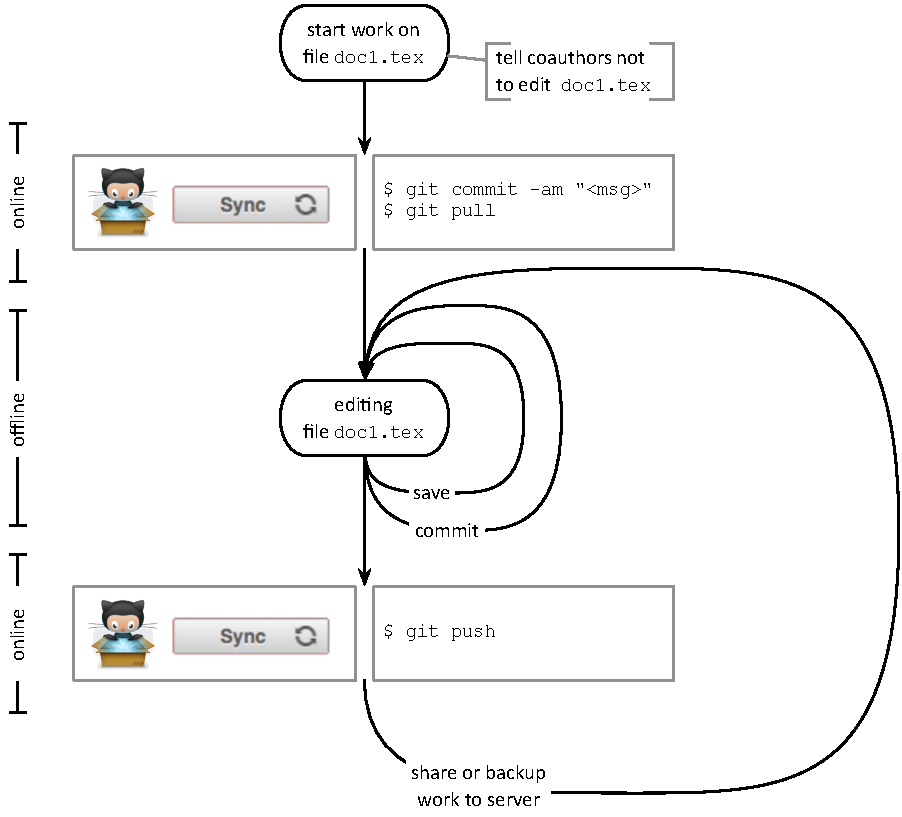
\includegraphics[width=\textwidth,height=.3\textheight,keepaspectratio]{figures/workcycle}
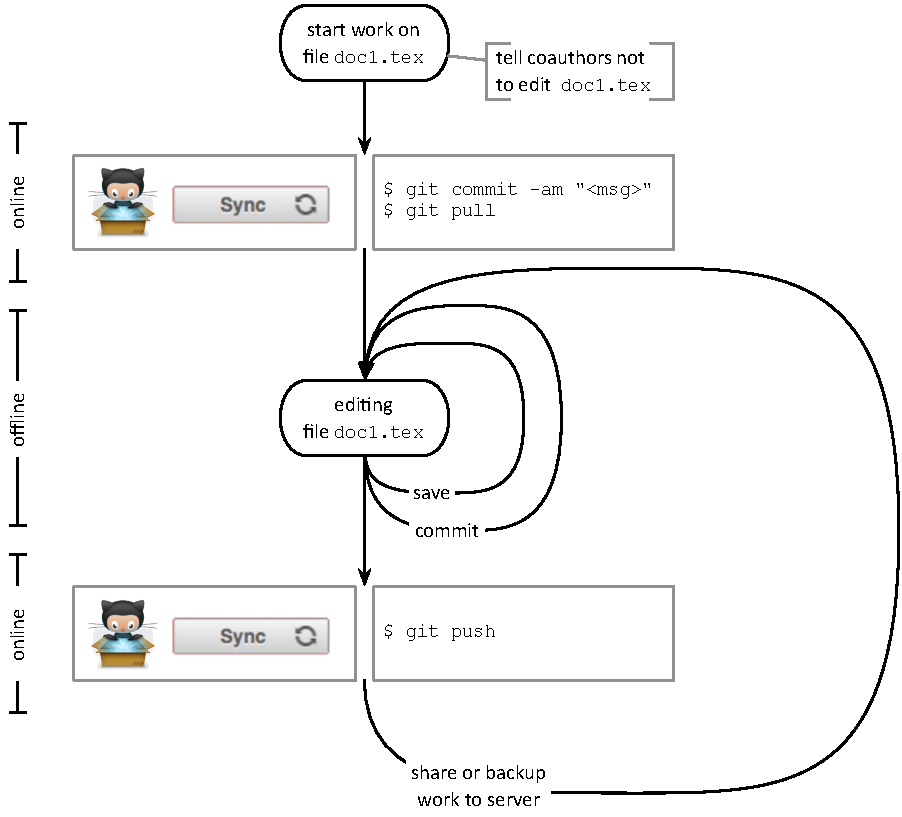
\includegraphics{figures/workcycle.pdf}
\caption{Typical work cycle for shared writing project} \label{fig:work cycle}
\end{figure}

